\documentclass[tikz]{standalone}

\usepackage{pgfplots}
\pgfplotsset{compat=1.15}
\usepackage{mathrsfs}
\usetikzlibrary{arrows,calc}
\usepackage{tkz-euclide}
\pagestyle{empty}

\definecolor{AngleClr}{rgb}{0,0.39215686274509803,0}
\definecolor{ShapeClr}{rgb}{0.6,0.2,0}

\begin{document}

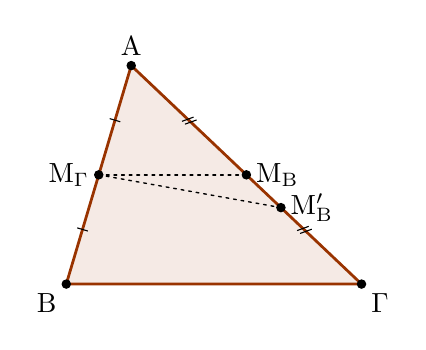
\begin{tikzpicture}[scale=.75]
\tkzSetUpLine[line width=1pt,color=black]
\tkzSetUpPoint[fill=black]

\tkzDefPoints{0/0/B,1.1/3.7/A,5/0/C}

\tkzDefMidPoint(A,B) \tkzGetPoint{MC}
\tkzDefMidPoint(A,C) \tkzGetPoint{MB}

\tkzDefPointOnLine[pos=0.65](A,C)\tkzGetPoint{MB'}

\tkzFillPolygon[fill=ShapeClr,fill opacity=0.1](A,B,C)

\tkzDrawSegments[line width=0.5pt,color=black,dashed,dash pattern=on 1pt off 1.75pt](MC,MB MC,MB')

\tkzDrawPolygon[color=ShapeClr](A,B,C)
\tkzDrawPoints[size=3](A,B,C,MB,MB',MC)

\tkzLabelPoint[above](A){$\rm A$}
\tkzLabelPoint[below left](B){$\rm B$}
\tkzLabelPoint[below right](C){$\rm \Gamma$}

\tkzLabelPoint[right](MB){$\rm M_B$}
\tkzLabelPoint[right](MB'){$\rm M_B'$}
\tkzLabelPoint[left](MC){$\rm M_\Gamma$}

\tkzMarkSegments[mark=|,size=2](A,MC MC,B)
\tkzMarkSegments[mark=s||,size=2](A,MB MB,C)


\end{tikzpicture}

\end{document}
